\section{Particle Identification}\label{sec:analysis.pid}
	Lepton identification was based on conservation of mass. Once the data is skimmed according to Table~\ref{tab:skim.requirements}, all particles that were $\pi^+$, $\pi^-$, 
	unknown with $q^+$ or unknown with $q^-$ were tentatively assigned to be electrons or positrons based on their charge. 
	\subsection{Kinematic Cuts}\label{sec:analysis.cuts}
		First it should be noted that for the /g12 experiment, there was a two-prong trigger for events in which the photon beam energy was greater then 3.6~GeV, while for the 
		entire data taking process there was a ``lepton'' trigger configuration. Therefore to measure the differential cross-section at photon beam energies less than 3.6~GeV this 
		``lepton'' trigger information was employed. 
		Once particle section was achieved, it was necessary to reduce the background of the exclusive $\gamma p \to p \pi^{+}\pi^{-}$ reaction. For events of photon beam 
		energy less than 3.6~GeV, a \abbr{CC} and \abbr{EC} ``hit'' must have been recorded for each charge track that was not the proton. For all events 3 kinematic fits were 
		performed, a 1-C ( $\gamma p \to p e^{+}e^{-}(\gamma)$) to identify the missing photon in the reaction, a 4-C ($\gamma p \to p \pi^{+}\pi^{-}$) as a discriminator and a 
		2-C ($\gamma p \to p \pi^0 \to pe^{+}e^{-}(\gamma)$) to identify the reaction. After the kinematic fit, a 1\% confidence level cut was placed on the 1-C fit. The missing 
		energy of the $\gamma p \to p e^{+}e^{-}$ spectrum versus the missing mass of $\gamma p \to p X$ was analyzed and shown that a 75~MeV cut on the missing energy 
		was suitable to suppress the $\gamma p \to p \pi^{+}\pi^{-}$ reaction. After the missing energy cut, the signal to background ratio was $\sim 99.7\%$, see right 
		figure~\ref{fig:Mxp}, the other 4-C and 2-C fits were then used with a 1\% confidence on each to suppress the background to $\sim 99.9\%$.
		\begin{figure}[h!]\begin{center}
				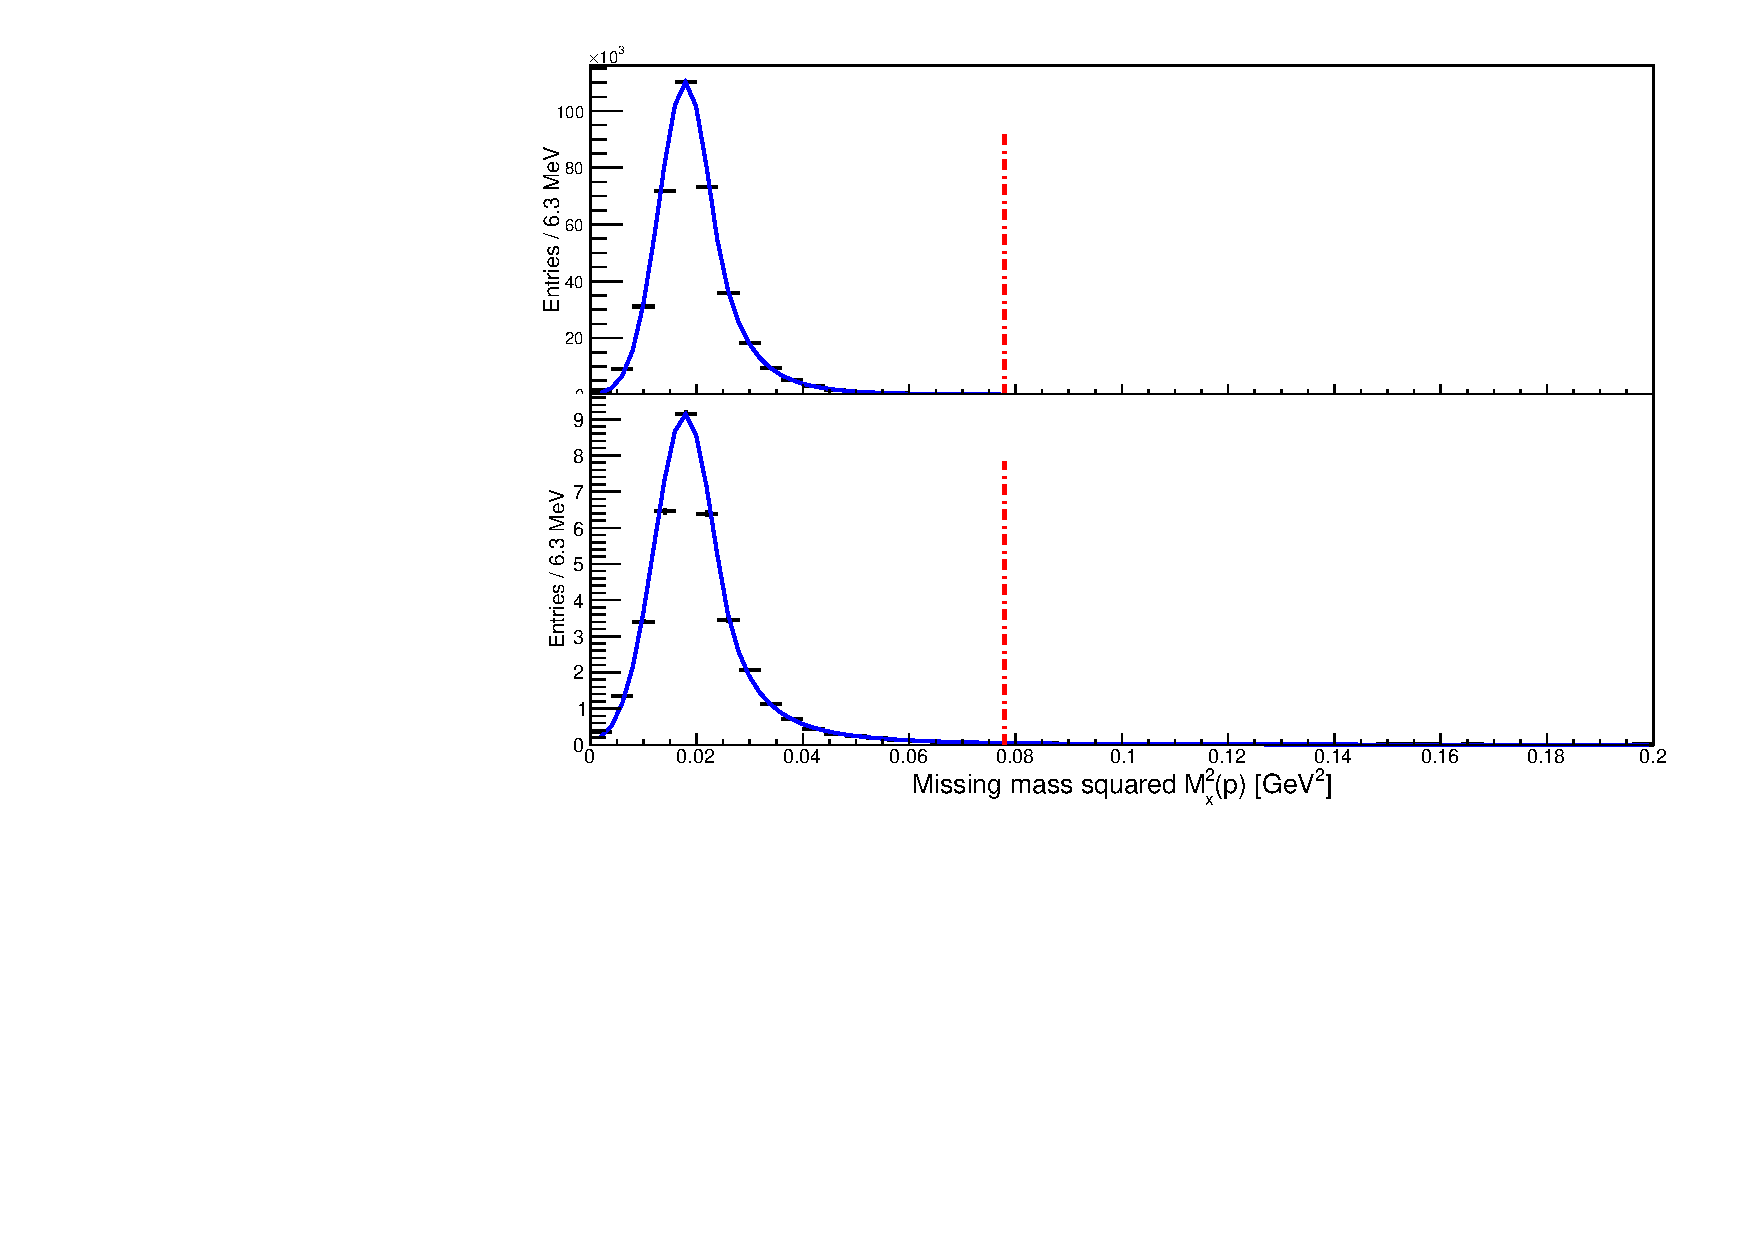
\includegraphics[width=270 pt, height=200 pt]{\figures/DATA/hdataLEP_MOR_pi0_FINAL_PLOTS_nolabel.pdf}		
				\caption{(Black points)$M_x^2(p)$ data used in analysis. (Blue line) Fit using Crystal Ball function. The horizontal red dashed-dotted line depicts the threshold of $\pi^{+}\pi^{-}$ production. Top:Data for photon energies below 3.6~GeV. Bottom:Data for beam photon energies greater than 3.6~GeV}{}
				\label{fig:Mxp}
		\end{center}\end{figure}